\chapter{Technology Review}
This chapter discusses the different technologies used in throughout the
project. It discusses the the advantages and disadvantages of each technology 
and why certain technologies were used over others. It also discusses hybrid applications compared to native applications, advantages, disadvantages, uses at different business structures and other topics.

\section{Overview}
This project is a Native android app built with Kotlin in Android Studio, Firebase is used for the database, statistics, verification etc.

Topics:
\begin{itemize}
    \item Kotlin/Java comparison
    \item Fire-base
    \item Picasso
    \item Android Studio/IntelliJ
    \item Native Applications
    \item Hybrid Applications
    \item Hybrid vs Native comparison 
\end{itemize}
\newpage

\section{Main Technologies}
This section will discuss the main technologies currently in use in the android application.

\subsection{Kotlin}
\par
\medskip
\begin{center}
    
\includegraphics[width=12cm,height=12cm,keepaspectratio]{Images/Kotlin.png}
\end{center}
Kotlin is a cross-platform, statically typed, general-purpose programming language with type inference. Kotlin is designed to inter-operate fully with Java, and the JVM version of its standard library depends on the Java Class Library, but type inference allows its syntax to be more concise. Kotlin mainly targets the JVM, but also compiles to JavaScript or native code (via LLVM). Language development costs are borne by JetBrains, while the Kotlin Foundation protects the Kotlin trademark.

Kotlin is the preferred language for Android app developers as of May 2019, since the release of Android Studio 3.0 in October 2017, Kotlin has been included as an alternative to the standard Java compiler. The Android Kotlin compiler targets Java 6 by default, and lets programmers choose between Java 8 to 14 for optimization purposes.

Kotlin originated at JetBrains, which is the company behind IntelliJ IDEA. Kotlin has been open source since 2012 and has a large team of full-time developers working on it, there is also the \hyperlink{https://github.com/JetBrains/kotlin}{Kotlin project of GitHub} which has more than 370 contributors.

\newpage

\subsubsection{Advantages}
Kotlin has many advantages, many are quite serious improvements in readability and workflow which was noticeable when creating my project

\begin{itemize}
    \item \textbf{Less code combined with greater readability} - Spend less time writing code and working to understand the code of others.
    \item \textbf{Mature language and environment} - Kotlin has developed continuously over the years not only as a language but as a whole ecosystem with very robust tooling. Its seamless integration with Android Studio, makes it actively used by companies to develop Android applications.
    \item \textbf{Kotlin support of Android Jetpack and other libraries} - \hyperlink{https://developer.android.com/kotlin/ktx}{KTX extensions} adds kotlin language features, such as coroutines, extension functions, lambdas, and named parameters, to existing Android libraries.
    \item \textbf{Interoperability with Java} - You can use Kotlin along with the Java programming language in your applications without needing to migrate all your code to Kotlin. 
    \item \textbf{Support for multi-platform development} - You can use Kotlin for developing not only Android but also iOS, back-end, and web applications by sharing the common code among the platforms.
    \item \textbf{Code safety} - Less code and better readability lead to fewer errors. The Kotlin compiler detects the remaining errors, making the code safe. 
    \item \textbf{Easy to Learn} - Kotlin is very easy to learn, especially for any Java experienced developers. 
    \item \textbf{Large community} - Kotlin a great support and many contributions from the community, which is growing all over the world. According to Google, over 60\% of the top 100 apps on the Google Play Store use Kotlin. Many startups and Fortune 500 companies have already developed Android applications using Kotlin and more and more companies are prioritizing Kotlin Native application development over other options due to the robust toolkit and optimizations that make your applications the best that they can be. 
\end{itemize}

\newpage

\subsubsection{Disadvantages}

\begin{itemize}
    \item \textbf{Shift from Java to Kotlin} - Kotlin is an amazing programming language and there is a reason why leading lead companies have started using kotlin, but at their core their two different languages. Developers won't be able to quickly shift from one to another without taking time to learn Kotlin. Therefore company's have to consider different approaches to Android app development as additional expenses are required on training a team of developers. 
    \item \textbf{Hard to find experienced developers} - There is a high demand for specialists in Kotlin as Google made it the preferred language for Android development in 2019, but there is still a very large amount of Java programmers on the market compared to Kotlin developers. This means on average the Kotlin developers may be younger meaning less senior developers available for hire. This is quite a large disadvantage, but will quickly fade away as many leading tech companies have switched which creates a ripple effect down the chain of companies.
    \item \textbf{Limited learning resources} - Although the number of Android app developers who use Kotlin instead of Java increase everyday, there is still a limited number of resources in the market compared to Java. Many College courses will teach Java over Kotlin as both are so similar, meaning most Kotlin developers come from a background in Java and learn to code in Kotlin themselves.
\end{itemize}

\newpage
\subsubsection{Kotlin Syntax}
Kotlin syntax is familiar to any programmer that is from a OOP domain and be be more or less understood from the get-go. There are differences from Java such as primary and secondary constructors, val \& var variable declarations and more.
\newline

\textbf{Below you can see the basic structure of a class in kotlin}
\begin{lstlisting}
class Foo {

    val b: String = "b"     // val means unmodifiable
    var i: Int = 0          // var means modifiable

    fun hello() {
        val str = "Hello"
        print("$str World")
    }

    fun sum(x: Int, y: Int): Int {
        return x + y
    }

    fun maxOf(a: Float, b: Float) = if (a > b) a else b

}
\end{lstlisting}

\textbf{String Interpolation} - A smarter and more readable version of Java's String.format() that is built into the language
\begin{lstlisting}
val x = 5
val y = 10
print("sum of $x and $y is ${x + y}")  // sum of 5 and 10 is 15
\end{lstlisting}

\textbf{Type Inference} - Kotlin will infer your types wherever you feel it will improve readability
\begin{lstlisting}
val a = "abc"                         // type inferred to String
val b = 4                             // type inferred to Int

val c: Double = 0.7                   // type declared explicitly
val d: List<String> = ArrayList()     // type declared explicitly
\end{lstlisting}

\textbf{Smart Casts} - The Kotlin compiler tracks logic and auto-casts types if possible, which means you do not need to use instanceof checks followed by explicit casts
\begin{lstlisting}
if (obj is String) {
    print(obj.toUpperCase())     // obj is now known to be a String
}
\end{lstlisting}

\textbf{When Expression} - The switch case is replaced with the more readable and flexible when() expression
\begin{lstlisting}
when (x) {
    1 -> print("x is 1")
    2 -> print("x is 2")
    3, 4 -> print("x is 3 or 4")
    in 5..10 -> print("x is 5, 6, 7, 8, 9, or 10")
    else -> print("x is out of range")
}

// It also works as an expression or a statement
// with or without an argument
val res: Boolean = when {
    obj == null -> false
    obj is String -> true
    else -> throw IllegalStateException()
}
\end{lstlisting}

\textbf{Setter \& Getter behavior} - You can make custom set \& get behaviors that are added to public fields, which means getter \& setters won't bloat your code
\begin{lstlisting}
class Frame {
    var width: Int = 800
    var height: Int = 600

    val pixels: Int
        get() = width * height
}
\end{lstlisting}

\textbf{Data Classes} - We frequently create classes whose main purpose is to hold data. In such a class some standard functionality and utility functions are often mechanically derivable from the data. In kotlin, this is called a data class and is marked as data. Its a Plain Old Java Object so its complete with toString(), equals(), hashCode() and copy().
\begin{lstlisting}
data class Person(val name: String,
                  var email: String,
                  var age: Int)

val john = Person("John", "john@gmail.com", 112)
}
\end{lstlisting}

\subsection{Kotlin vs Java}
\par
\medskip
\begin{center}
    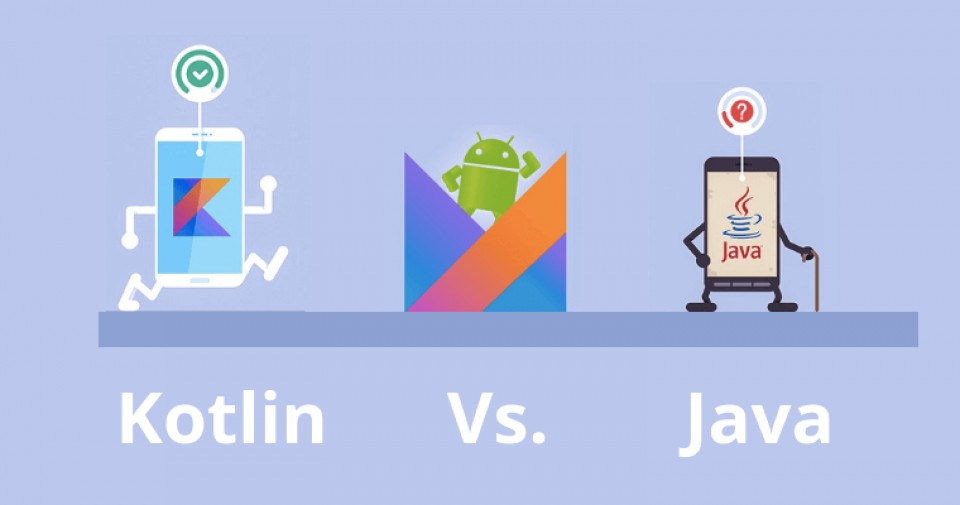
\includegraphics[width=12cm,height=12cm,keepaspectratio]{Images/KotlinvJava.jpg}
\end{center}

blah..


\subsubsection{Advantages}
\begin{itemize}
    \item \textbf{Shift from Java to Kotlin} - Kotlin
    \item \textbf{Hard to find experienced developers} - asdas
    \item \textbf{Limited learning resources} - Although
\end{itemize}
\subsubsection{Disadvantages}
\begin{itemize}
    \item \textbf{Shift from Java to Kotlin} - Kotlin
    \item \textbf{Hard to find experienced developers} - asdas
    \item \textbf{Limited learning resources} - Although
\end{itemize}

\newpage
\subsection{Firebase}
\par
\medskip
\begin{center}
    
\includegraphics[width=12cm,height=12cm,keepaspectratio]{Images/firebase.png}
\end{center}

Firebase is Google's mobile and web application development platform that helps you build, improve, and grow your application. Firebase frees developers to focus on crafting excellent user experiences. You don't need to manage servers. You don't need to write APIs. Firebase is your server, your API and your database, everything is written generically so that you can modify everything to suit most needs. Firebase has a huge amount of features, real time databases, cloud storage, hosting, machine learning, authentication, statistics, analytics and more.\newline

Firebase products are setup in three different area's. Build better apps, Improve app quality \& Grow your business

\subsubsection{Build better apps} Firebase lets you build more powerful, secure and scalable apps, using world-class infrastructure. There are seven different products focused on building a better app. My project takes advantage of Authenication, Realtime Database and Cloud storage. Almost all of Firebase products are extremely useful and are worth mentioning as they could be implemented into the project at some point.
I will first summarize the products, and then go into further detail on the specific products i used in my project. How the code is implemented, why i used it etc.

\newpage
\subsubsection{Products for building better apps}
\begin{itemize}
    \item \textbf{Cloud Firestore} - Store and sync data between users and devices - at global scale - using a cloud-hosted, NOSQL database. Cloud Firestore gives you live synchronization and offline support along with efficient data queries. Its integration with other Firebase products enables you to build truly serverless apps.
    \item \textbf{ML Kit} - Bring powerful machine learning features to your mobile app whether you're new or experienced in ML. Get started easily by using our ready-to-use APIs for common mobile use cases, or import your own custom models which can be hosted and served to your apps by Firebase. ML Kit APIs can run on-device or in the cloud, depending on the functionality, and some give you both choices.
    \item \textbf{Cloud Functions} - Extend your app with custom backend code without needing to manage and scale your own servers. Functions can be triggered by events, which are emitted by Firebase products, Google Cloud services, or third parties, using webhook
    \item \textbf{Authentication} - Manage your users in a simple and secure way. Firebase Auth offers multiple methods to authenticate, including email and password, third-party providers like Google or Facebook, and using your existing account system directly. Build your own interface, or take advantage of our open source, fully customizable UI.
    \item \textbf{Hosting} - Simplify your web hosting with tools made specifically for modern web apps. When you upload your web assets, we automatically push them out to our global CDN and give them a free SSL certificate so your users get a secure, reliable, low-latency experience, no matter where they are.
    \item \textbf{Cloud Storage} - Store and share user-generated content like images, audio, and video with powerful, simple, and cost-effective object storage built for Google scale. The Firebase SDKs for Cloud Storage add Google security to file uploads and downloads for your Firebase apps, regardless of network quality.
    \item \textbf{Realtime Database} - Realtime Database is Firebase's original database. It's an efficient, low-latency solution for mobile apps that require synced states across clients in realtime. We recommend Cloud Firestore instead of Realtime Database for most developers starting a new project.
\end{itemize}

\newpage
\subsubsection{Improve app quality}
Firebase gives you insights into app performance and stability, so you can channel your resources effectively.
These products weren't used in the project, but are worth mentioning as they are quite valuable in a commercial development environment where app performance and crashing have a huge impact on user
\subsubsection{Grow your business}
aaa
\begin{center}
    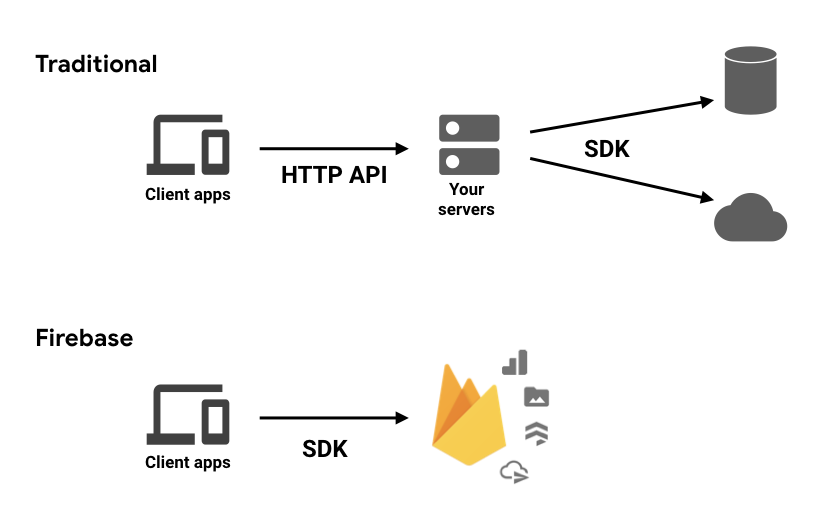
\includegraphics[width=12cm,height=12cm,keepaspectratio]{Images/firebasetradpic.png}
\end{center}


\subsubsection{Advantages}
\begin{itemize}
    \item \textbf{Shift from Java to Kotlin} - Kotlin
    \item \textbf{Hard to find experienced developers} - asdas
    \item \textbf{Limited learning resources} - Although
\end{itemize}
\subsubsection{Disadvantages}
\begin{itemize}
    \item \textbf{Shift from Java to Kotlin} - Kotlin
    \item \textbf{Hard to find experienced developers} - asdas
    \item \textbf{Limited learning resources} - Although
\end{itemize}
\subsection{Picasso}
\par
\medskip
\begin{center}
    
\includegraphics[width=10cm,height=10cm,keepaspectratio]{Images/picasso.png}
\end{center}

blah..


\subsubsection{Advantages}
\begin{itemize}
    \item \textbf{Shift from Java to Kotlin} - Kotlin
    \item \textbf{Hard to find experienced developers} - asdas
    \item \textbf{Limited learning resources} - Although
\end{itemize}
\subsubsection{Disadvantages}
\begin{itemize}
    \item \textbf{Shift from Java to Kotlin} - Kotlin
    \item \textbf{Hard to find experienced developers} - asdas
    \item \textbf{Limited learning resources} - Although
\end{itemize}

\subsection{Native Applications}
\par
\medskip
\begin{center}
    
\includegraphics[width=12cm,height=12cm,keepaspectratio]{Images/nativeapp2.png}
\end{center}

blah..


\subsubsection{Advantages}
\begin{itemize}
    \item \textbf{Shift from Java to Kotlin} - Kotlin
    \item \textbf{Hard to find experienced developers} - asdas
    \item \textbf{Limited learning resources} - Although
\end{itemize}
\subsubsection{Disadvantages}
\begin{itemize}
    \item \textbf{Shift from Java to Kotlin} - Kotlin
    \item \textbf{Hard to find experienced developers} - asdas
    \item \textbf{Limited learning resources} - Although
\end{itemize}

\subsection{Hybrid Applications}
\par
\medskip
\begin{center}
    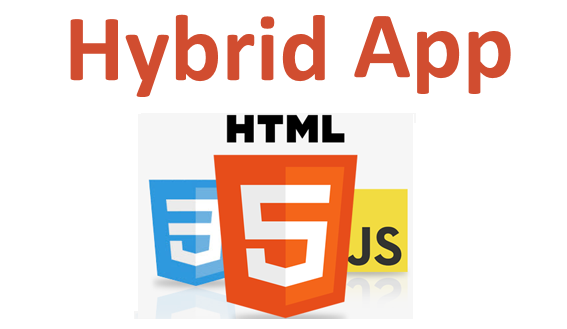
\includegraphics[width=12cm,height=12cm,keepaspectratio]{Images/hybridapp.png}
\end{center}

blah..


\subsubsection{Advantages}
\begin{itemize}
    \item \textbf{Shift from Java to Kotlin} - Kotlin
    \item \textbf{Hard to find experienced developers} - asdas
    \item \textbf{Limited learning resources} - Although
\end{itemize}
\subsubsection{Disadvantages}
\begin{itemize}
    \item \textbf{Shift from Java to Kotlin} - Kotlin
    \item \textbf{Hard to find experienced developers} - asdas
    \item \textbf{Limited learning resources} - Although
\end{itemize}

\subsection{Hybrid vs Native Applications}
\par
\medskip
\begin{center}
    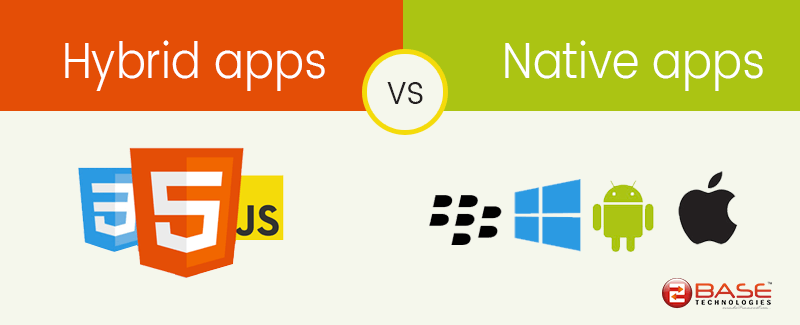
\includegraphics[width=12cm,height=12cm,keepaspectratio]{Images/hybridvnative.png}
\end{center}

blah..


\subsubsection{Advantages}
\begin{itemize}
    \item \textbf{Shift from Java to Kotlin} - Kotlin
    \item \textbf{Hard to find experienced developers} - asdas
    \item \textbf{Limited learning resources} - Although
\end{itemize}
\subsubsection{Disadvantages}
\begin{itemize}
    \item \textbf{Shift from Java to Kotlin} - Kotlin
    \item \textbf{Hard to find experienced developers} - asdas
    \item \textbf{Limited learning resources} - Although
\end{itemize}

\begin{figure}[h!]
	\caption{Hybrid Application}
	\label{image:myImageName}
	\centering
	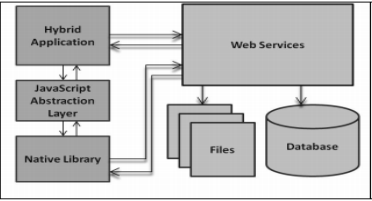
\includegraphics[width=1\textwidth]{Images/hybrid_dev_img.PNG}
\end{figure}
